% Options for packages loaded elsewhere
\PassOptionsToPackage{unicode}{hyperref}
\PassOptionsToPackage{hyphens}{url}
\PassOptionsToPackage{dvipsnames,svgnames,x11names}{xcolor}
%
\documentclass[
  letterpaper,
  DIV=11,
  numbers=noendperiod]{scrartcl}

\usepackage{amsmath,amssymb}
\usepackage{iftex}
\ifPDFTeX
  \usepackage[T1]{fontenc}
  \usepackage[utf8]{inputenc}
  \usepackage{textcomp} % provide euro and other symbols
\else % if luatex or xetex
  \usepackage{unicode-math}
  \defaultfontfeatures{Scale=MatchLowercase}
  \defaultfontfeatures[\rmfamily]{Ligatures=TeX,Scale=1}
\fi
\usepackage{lmodern}
\ifPDFTeX\else  
    % xetex/luatex font selection
\fi
% Use upquote if available, for straight quotes in verbatim environments
\IfFileExists{upquote.sty}{\usepackage{upquote}}{}
\IfFileExists{microtype.sty}{% use microtype if available
  \usepackage[]{microtype}
  \UseMicrotypeSet[protrusion]{basicmath} % disable protrusion for tt fonts
}{}
\makeatletter
\@ifundefined{KOMAClassName}{% if non-KOMA class
  \IfFileExists{parskip.sty}{%
    \usepackage{parskip}
  }{% else
    \setlength{\parindent}{0pt}
    \setlength{\parskip}{6pt plus 2pt minus 1pt}}
}{% if KOMA class
  \KOMAoptions{parskip=half}}
\makeatother
\usepackage{xcolor}
\setlength{\emergencystretch}{3em} % prevent overfull lines
\setcounter{secnumdepth}{-\maxdimen} % remove section numbering
% Make \paragraph and \subparagraph free-standing
\makeatletter
\ifx\paragraph\undefined\else
  \let\oldparagraph\paragraph
  \renewcommand{\paragraph}{
    \@ifstar
      \xxxParagraphStar
      \xxxParagraphNoStar
  }
  \newcommand{\xxxParagraphStar}[1]{\oldparagraph*{#1}\mbox{}}
  \newcommand{\xxxParagraphNoStar}[1]{\oldparagraph{#1}\mbox{}}
\fi
\ifx\subparagraph\undefined\else
  \let\oldsubparagraph\subparagraph
  \renewcommand{\subparagraph}{
    \@ifstar
      \xxxSubParagraphStar
      \xxxSubParagraphNoStar
  }
  \newcommand{\xxxSubParagraphStar}[1]{\oldsubparagraph*{#1}\mbox{}}
  \newcommand{\xxxSubParagraphNoStar}[1]{\oldsubparagraph{#1}\mbox{}}
\fi
\makeatother


\providecommand{\tightlist}{%
  \setlength{\itemsep}{0pt}\setlength{\parskip}{0pt}}\usepackage{longtable,booktabs,array}
\usepackage{calc} % for calculating minipage widths
% Correct order of tables after \paragraph or \subparagraph
\usepackage{etoolbox}
\makeatletter
\patchcmd\longtable{\par}{\if@noskipsec\mbox{}\fi\par}{}{}
\makeatother
% Allow footnotes in longtable head/foot
\IfFileExists{footnotehyper.sty}{\usepackage{footnotehyper}}{\usepackage{footnote}}
\makesavenoteenv{longtable}
\usepackage{graphicx}
\makeatletter
\def\maxwidth{\ifdim\Gin@nat@width>\linewidth\linewidth\else\Gin@nat@width\fi}
\def\maxheight{\ifdim\Gin@nat@height>\textheight\textheight\else\Gin@nat@height\fi}
\makeatother
% Scale images if necessary, so that they will not overflow the page
% margins by default, and it is still possible to overwrite the defaults
% using explicit options in \includegraphics[width, height, ...]{}
\setkeys{Gin}{width=\maxwidth,height=\maxheight,keepaspectratio}
% Set default figure placement to htbp
\makeatletter
\def\fps@figure{htbp}
\makeatother

\KOMAoption{captions}{tableheading}
\makeatletter
\@ifpackageloaded{caption}{}{\usepackage{caption}}
\AtBeginDocument{%
\ifdefined\contentsname
  \renewcommand*\contentsname{Table of contents}
\else
  \newcommand\contentsname{Table of contents}
\fi
\ifdefined\listfigurename
  \renewcommand*\listfigurename{List of Figures}
\else
  \newcommand\listfigurename{List of Figures}
\fi
\ifdefined\listtablename
  \renewcommand*\listtablename{List of Tables}
\else
  \newcommand\listtablename{List of Tables}
\fi
\ifdefined\figurename
  \renewcommand*\figurename{Figure}
\else
  \newcommand\figurename{Figure}
\fi
\ifdefined\tablename
  \renewcommand*\tablename{Table}
\else
  \newcommand\tablename{Table}
\fi
}
\@ifpackageloaded{float}{}{\usepackage{float}}
\floatstyle{ruled}
\@ifundefined{c@chapter}{\newfloat{codelisting}{h}{lop}}{\newfloat{codelisting}{h}{lop}[chapter]}
\floatname{codelisting}{Listing}
\newcommand*\listoflistings{\listof{codelisting}{List of Listings}}
\makeatother
\makeatletter
\makeatother
\makeatletter
\@ifpackageloaded{caption}{}{\usepackage{caption}}
\@ifpackageloaded{subcaption}{}{\usepackage{subcaption}}
\makeatother

\ifLuaTeX
  \usepackage{selnolig}  % disable illegal ligatures
\fi
\usepackage{bookmark}

\IfFileExists{xurl.sty}{\usepackage{xurl}}{} % add URL line breaks if available
\urlstyle{same} % disable monospaced font for URLs
\hypersetup{
  pdftitle={QTM 350 Final Project: Finding the Key to GDP Growth in Developing, Transitionary and Developed Nations},
  pdfauthor={Olivia Moody (2519203), Minsol Kim (2495685), and Simon Liu (2487435)},
  colorlinks=true,
  linkcolor={blue},
  filecolor={Maroon},
  citecolor={Blue},
  urlcolor={Blue},
  pdfcreator={LaTeX via pandoc}}


\title{QTM 350 Final Project: Finding the Key to GDP Growth in
Developing, Transitionary and Developed Nations}
\author{Olivia Moody (2519203), Minsol Kim (2495685), and Simon Liu
(2487435)}
\date{December 8, 2024}

\begin{document}
\maketitle


\subsection{Introduction}\label{introduction}

As transportation, technology and media advance at breaknecking speed,
the world's economies have become significantly more interconnected and
global than ever before. While many countries have been able to use
these advancements to aid in their development, many others are still in
transitionary or developing stages and find themselves with imbalanced
imports and exports. In order evaluate economic change over time, we
sought to explore the metric of GDP growth rate in developing and
developed countries over time. More specifically, we wanted to answer
the question: Are economic and educational attainment metrics correlated
with increased GDP growth rate? Is this correlation found in both
developed and developing countries? For this analysis we focused on the
the relationship between unemployment rate, inflation rate, and
government expenditure on education to GDP growth rate. Then we examined
the potential for collinearity (confounding variables), using a
correlation matrix, of all nine extracted independent economic and
educational variables.

Overall, we found that inflation rate was the only metric that had a
positive correlation to GDP growth rate and that it was somewhat
consistent on in developing and developed countries. While unemployment
rate had a negative correlation to GDP growth rate for both types of
economies, it had a much larger correlation for developing countries.
Finally, government expenditures on education had a negative correlation
with GDP Growth Rate only in developing countries but almost no
correlation on average in developed countries. In our analysis of
independent health and education variables, we found that health factors
were signficantly more correlated with one another than educational
factors.

\subsection{Data Description}\label{data-description}

The data for this project originates from the public World Bank World
Development Indicators database. As an organization, the World Bank
seeks to provide key financial and educational assistant to in
developing countries' so that they may develop infrastructure and
advance economically. In support of their mission, the organization
collects reliable data from recognised international agencies and
organizations to produce the database used in this project. While the
World Bank has more than 1,600 indicators for 217 economies spanning as
far back as 1960, we focused on only nine indicators from the years of
2000 to 2022. These nine indicators span the topics of economics,
education, and population. In order to refine our research question and
specify our scope, we chose to complete our analysis on five developed
nations and 6 developing nations which can be shown in the table below.

\n  

\n    

\n      

Developed Countries

\n      

Developing Countries

\n    

\n  

\n  

\n    

\n      

United States of America

\n      

Russia

\n    

\n    

\n      

Australia

\n      

Brazil

\n    

\n    

\n      

United Kingdom

\n      

China

\n    

\n    

\n      

Germany

\n      

India

\n    

\n    

\n      

New Zealand

\n      

South Africa

\n    

\n    

\n      

\n      

Ethiopia

\n    

\n    

\n      

\n      

\n    

\n  

\n

We chose these nations as their economies repersent some of the largest
in the world and they take on a repersent a nuanced and wide definition
of the concept of a developing and developed nation. The two specific
countries we want to note in this analysis are China and Russia as they
are a case example of large, rich economies that often fall under a grey
zone of a transitionary economy. While many consider China and Russia
developed, both do not yet meet the conditions under the United Nations
to be developed. To understand this before we made our classifications,
we looked plotted each countries' GDP per capita from 1960 to now. As
You can see if the following graph, Russia and China fall very
similiarly historically but even still today with the other developing
countries of our study. While GDP per Capita is not the only significant
metric to a country's status as developed, we wanted to illustrate and
make clear our classifications and their foundings.

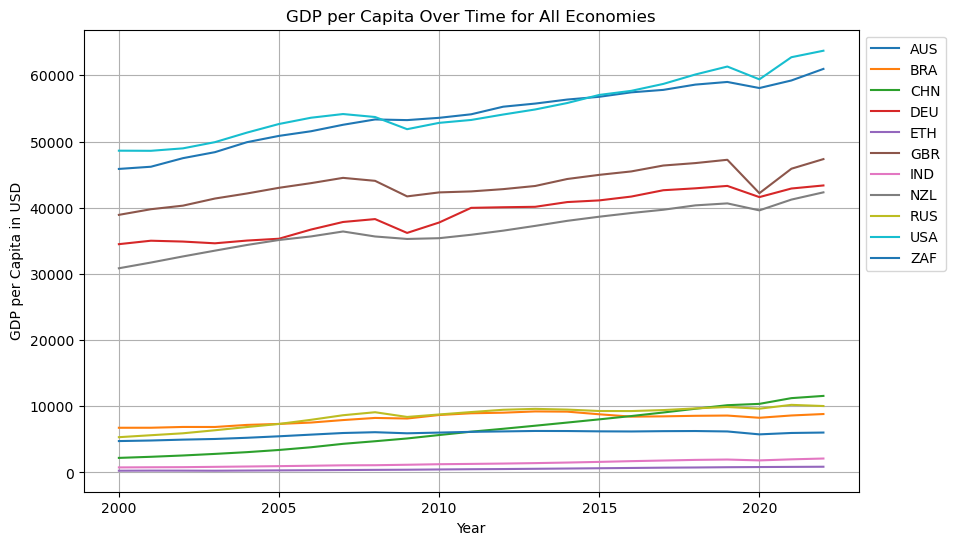
\includegraphics[width=1\textwidth,height=\textheight]{figures/GDP_per_Capita_Over_Time_for_All_Economies.png}

\subsubsection{Data Merging}\label{data-merging}

To complete our analysis we utilised SQL to extract four economic
indicators, three health indicators and three population indicators from
the World Bank's database. The following entity relationship diagram
shows this extraction and the usage of economy as a primary key amongst
them.

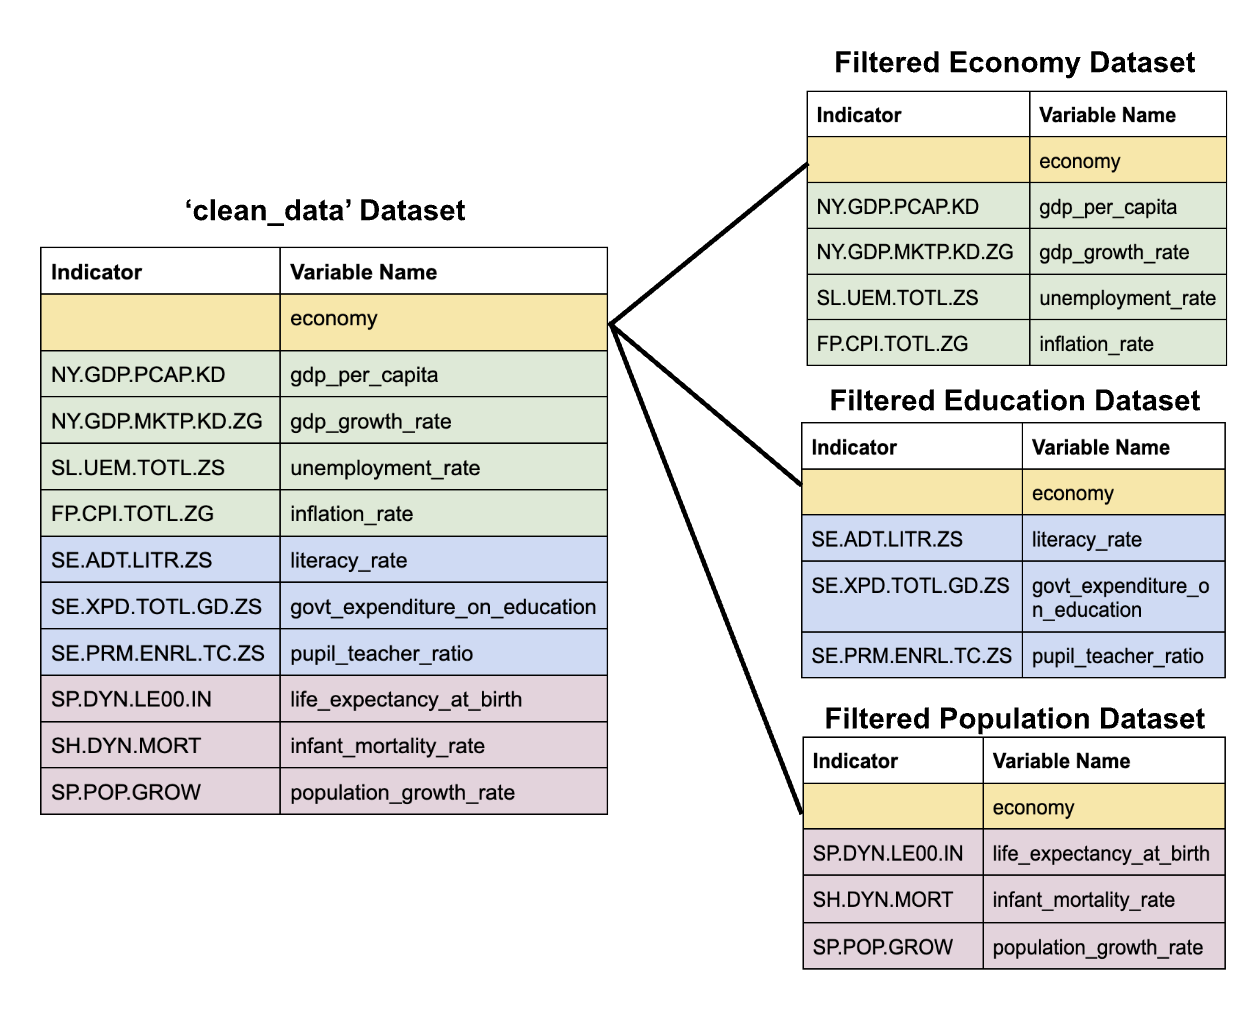
\includegraphics[width=1\textwidth,height=\textheight]{documentation/Entity_Relationship_Diagram.png}

\subsubsection{Data Cleaning and Pre-processing
Procedures}\label{data-cleaning-and-pre-processing-procedures}

While we extracted population variables, economic variables, and health
variables to evaluate variables most correlated with changes in GDP
growth rate over time, we quickly found in data cleaning that certain
variables were less usable than others. Specifically in developing
countries, the health and educational metrics often did not include
enough or completed time series data to preform our analysis. As a
result, we relied on a smaller set of key variables which had
statistical power.

\subsubsection{Key Variables}\label{key-variables}

The key variables relied upon in this paper were unemployment rate,
inflation rate, government expenditure on education, and GDP growth
rate.

\textbf{Unemployment Rate}: The unemployment rate measures the
percentage of the labor force that is actively seeking but unable to
find employment. Many see it as a proxy for the health of a country's
labor market and economy.

\textbf{Inflation Rate}: The inflation rate indicates the annual
percentage change in the average price level of goods and services in an
economy over a specific period. In other words, the inflation rate shows
how the purchasing power of a country's currency is changing over time.

\textbf{Government Expenditure on Education}: This indicator represents
the government's spending on the educational sector as a percentage of
the economy's GDP. The World Bank includes expenditures funded by
international sources to the government and defines government as
consisting of local, regional and central branches. Generally this
measure reflects the government's investment in human capital
development.

\textbf{GDP Growth Rate}: The GDP growth rate measures the annual
percentage change in a country's gross domestic product (GDP), which
indicates the overall economic growth or contraction of a country. The
World Bank defines this as the sum of gross value added by all resident
produces in the economy and product taxes minus subsidies otherwise not
included in products' values. It should be noted, especially for
developing countries which are often depended on for natural resources
and minerals, that the GDP and its growth rate does not reflect any
depreciation or damage of natural resources. GDP growth rate is thought
of as a key indicator of economic performance and stability.

\subsection{Data Analysis}\label{data-analysis}

To best visualise our results we have displayed all plots of developing
countries on the left and all plots of developed countries on the right.

\subsubsection{The Economic Story: Tracking Unemployment and Inflation
Rate to GDP Growth
Rate}\label{the-economic-story-tracking-unemployment-and-inflation-rate-to-gdp-growth-rate}

In term of economic indicators, the first key difference in our
aggregate of developing and developed economies is the range of GDP
growth rate, inflation rate and unemployment rate. As you can see in
both the plots below, the GDP growth rate takes on a slightly larger
range for our aggregate of developing countries. The more significant
trend, however is that the dispersal of points across the range is more
consistently varied in developing countries than developed ones. While
there is a few years of outliers in the developing countries, such as
Great Britain in 2008 reaching a horrific GDP growth rate below -10\%,
the devloped countries over time have a much tighter dispersal to one
another. We can also see this is in the error bands of the developing
countries being consistently thicker than the error bands of developed
countries. We can credit this to developing economies being both more
unique to each other than the grouping of developed nations as well as
the developing nations having larger changes economies through time. It
should be noted that in the same way developing nations sometimes had
large declines, they had similiarly high peaks unlike the developing
nations which almost never rose above a GDP growth rate above 5\% and
remained relatively stable through time.

The correlation between unemployment and GDP growth rate is negative in
both sets of economies but with a much larger correlation in developing
countries. Unlike the other metrics, which had a decently similiar
dispersal of the countries in each classification, South Africa (ZAF)
had a consistently much higher unemployment rate than the rest of the
developing countries. THis country also tended to be both much above and
much below the correlation line cementing its status as a outlier in the
data.

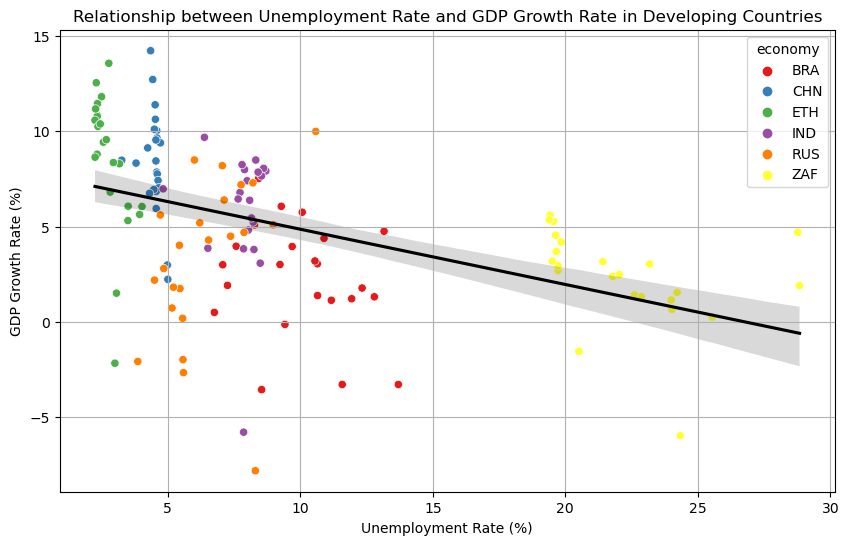
\includegraphics[width=0.45\textwidth,height=\textheight]{figures/Relationship_UnemploymentRate_GDPGrowthRate_DevelopingCountries.png}
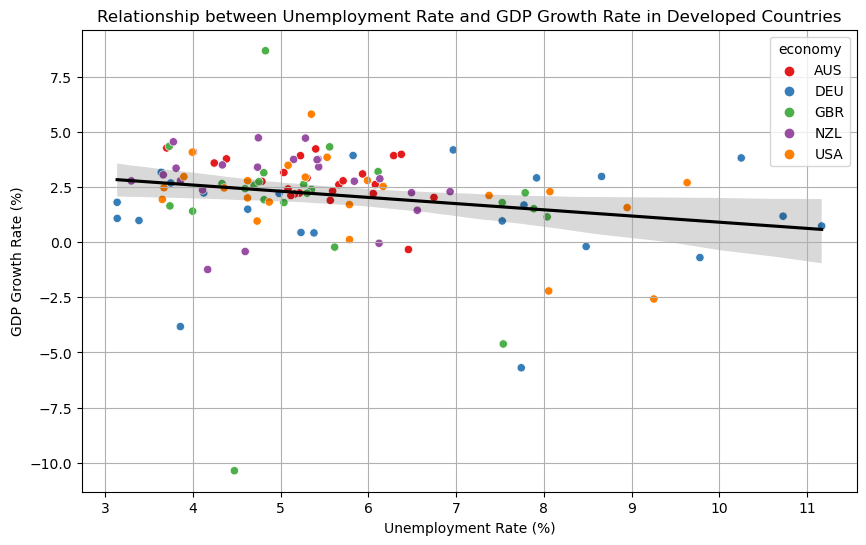
\includegraphics[width=0.45\textwidth,height=\textheight]{figures/Relationship_UnemploymentRate_GDPGrowthRate_Developed_Countries.png}

The correlation between annual inflation rate and GDP growth rate had a
slightly positive correlation in both developing and developed economies
with again much smaller error estimations for developing nations.
Inflation rate being a more consistent correlation across developed and
developing economies than unemployment rate could be explained by the
fact that inflation is influenced by broader macroeconomic factors, such
as monetary policy, global commodity prices, and supply-demand dynamics,
which tend to have more uniform effects across economies. In contrast,
unemployment is more closely tied to country-specific factors like labor
market conditions, structural issues, and social policies, which can
vary widely between developed and developing nations, leading to less
consistent correlations.

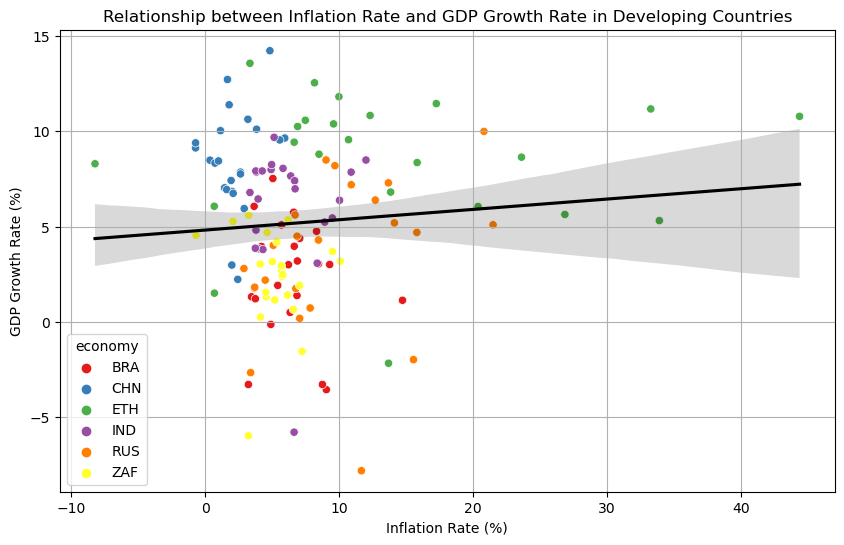
\includegraphics[width=0.45\textwidth,height=\textheight]{figures/Relationship_InflationRate_GDPGrowthRate_DevelopingCountries.png}
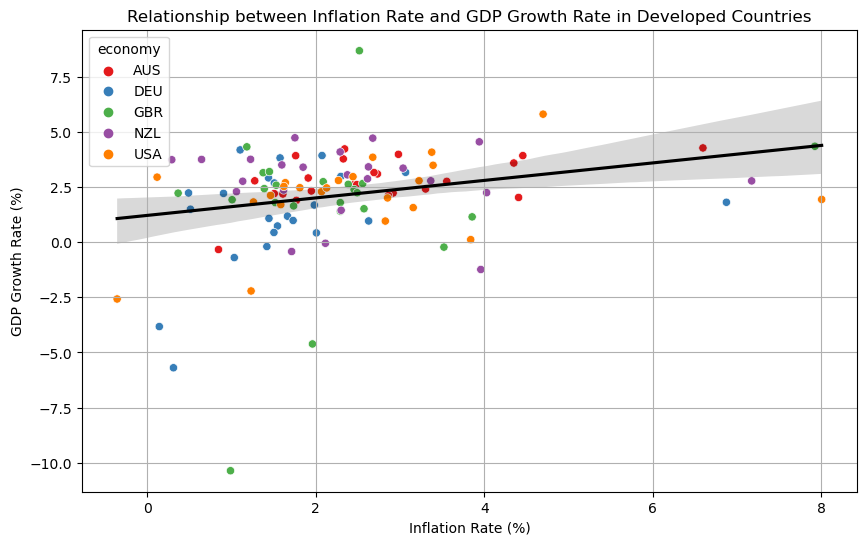
\includegraphics[width=0.45\textwidth,height=\textheight]{figures/Relationship_InflationRate_GDPGrowthRate_DevelopedCountries.png}

\subsubsection{The Education Story: Tracking Government Education
Expenditures and GDP Growth
Rate}\label{the-education-story-tracking-government-education-expenditures-and-gdp-growth-rate}

The correlation between government expenditures on education and GDP
growth rate was suprisingly negative in developing countries but neutral
in developed countries. This was the only indicator in which the range
was decently similiar among the two classifications, with government
expenditures making up between 2 and 7 percent in developing countries
and between about 4 and 7 percent in developing countries, which gives
added signficance to the different in trend between the educational and
economic metrics. A possible explanation for this trend could be that in
developing countries, government spending on education may not always be
efficiently allocated or may be hindered by structural issues such as
corruption, inadequate infrastructure, or a lack of educators, which
limits its impact on economic growth. In contrast, in developed
countries, education systems are generally more established and better
funded, leading to a more neutral relationship with GDP growth.

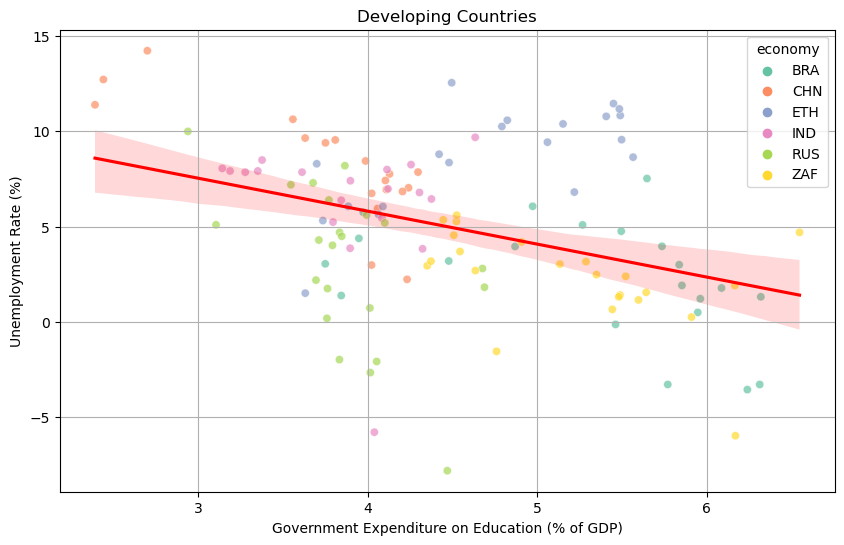
\includegraphics[width=0.45\textwidth,height=\textheight]{figures/GovernmentEducationExpenditures_GDPGrowthRate_Developing.png}
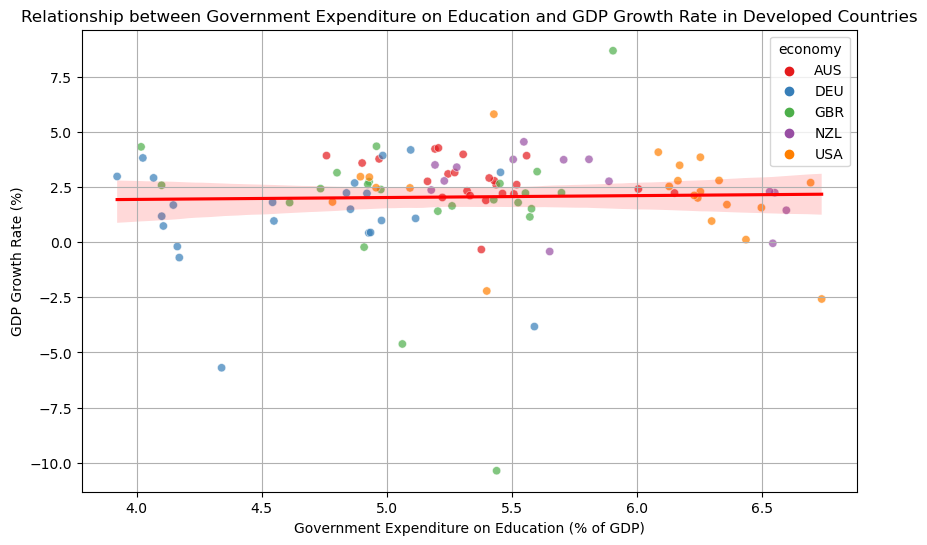
\includegraphics[width=0.45\textwidth,height=\textheight]{figures/GovernmentEducationExpenditures_GDPGrowthRate_Developed.png}

\subsubsection{Correlation Between Education, Economy and Health
Metrics}\label{correlation-between-education-economy-and-health-metrics}

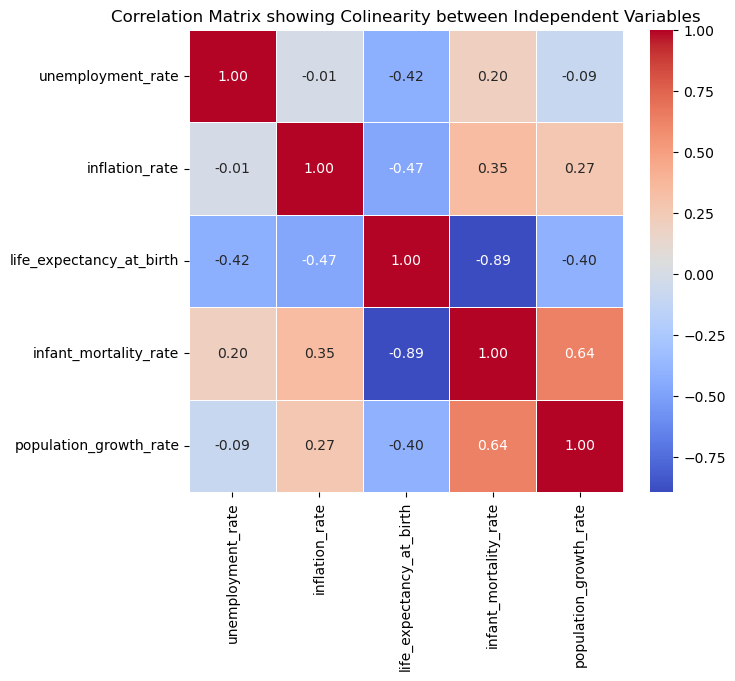
\includegraphics[width=1\textwidth,height=\textheight]{figures/CorrelationMatrix_Independent_Variables.png}

The indicators with the highest correlation between one another were
life expectancy at birth and infant mortality rate. This correlation was
-0.89 meaning that when infant mortality was increased, life expectancy
at birth was very commonly also decreased. The indicators with the
lowest correlation were inflation rate and unemployment rate which had a
very neutral correlation of -0.01.

\subsection{Results and Discussion}\label{results-and-discussion}

In summary, the data suggest that developing economies are much more
prone to economic volatility than developed ones, with higher growth
potential but also higher risks. While the negative correlation between
unemployment and GDP growth is consistent with economic theory, the
strength of this relationship varies, with developing countries
exhibiting more sensitivity to fluctuations. South Africa's outlier
status further highlights the complexity of unemployment trends in
developing countries, where factors like inequality, historical
legacies, and a limited labor market can significantly distort the
typical patterns seen in other emerging economies. Future research could
explore the specific explanations behind South Africa's high
unemployment rates and investigate whether similar patterns are
observable in other nations with comparable structural challenges.

While the results of educational investments to growth rate were
somewhat suprising as we often hear of education as a key to economic
sucess we must remember it is a very lagging indicator which will not
show economic impact immediately. In a developing country, a significant
portion of GDP growth may be driven by other factors, such as resource
extraction, which are less dependent on educational expenditures. While
education is crucial for long-term development, its immediate effect on
GDP growth may be less pronounced in developing countries compared to
their developed counterparts, where the link between education and
economic productivity may already be more fully realized.

In terms of indicator coorelation, we unsuprisingly found that health
indicators, such as infant mortality, life expectancy at birth, and
population growth rate, were correlated highest with each other. This
can be explained by the fact that a lot of these metrics are somehow
baked into one another or repersent a smaller subset of general health
indicators. For instance, if infant mortality rate as a percentage of
births is high, life expectancy at birth must be low by virtue of being
oppositional forces. In other words, the health indicators are a lot
less independent than the economic indicators.

Economic indicators were in general much less correlated with each other
which make sense in the general understanding that inflation rate is a
measure of change in currency value while unemployment rate is a measure
of change in available employment and human behavior. While they are
both heavily associated with the economy, they do not both boil down to
a identical root observation like the health metrics do to human life
span.

A key limitation of this study is its limited data to developing
countries. As described before many factors of health and education are
not able to be accurately studied as the World Bank does not have
reliable and consistent data through time of these countries. This has
large implications when we think of the power of data in telling a
country's stories. Without a sound story it is hard for organizations,
governments, and charities to accurately understand and meet
developmental needs. Particuarly in developing countries with little
governmental transparency, many markers of human development are hard to
follow through time and accurately gauge the effects of policy,
conflict, and environmental impacts. Utilising other data sources that
specialise on these countries could be a possible way of perservering
against this limitation in the future.

\subsection{Conclusion}\label{conclusion}

Overall the World Bank's Developmental Indicators is an amazing way to
find and study trends in different types of economies. While developing
countries economies are on average more subject to short term impacts,
they also have the largest room to grow in advance. Understanding the
key factors that lead to GDP growth rate is essential to making a path
towards a future where people in every region of the world can have
access to basic education, health, and opportunity.




\end{document}
